\documentclass[11pt]{article}

\usepackage[left=3.65cm,right=3.65cm,top=2.5cm,bottom=2.5cm]{geometry}
\usepackage{graphicx}
\usepackage[numbers]{natbib}
\usepackage{minted}   % syntax highlighting in code blocks
\usepackage{listings}
\usepackage{xcolor}
\usepackage[colorlinks=true, linkcolor=blue, urlcolor=blue, citecolor=blue]{hyperref}

\usepackage{microtype}  % nicer typesetting
\usepackage{newtxtext} % serif font for main body text
\usepackage{helvet} % sans serif font for headings/tables etc
\usepackage{inconsolata}  % font for comments in code blocks

\usepackage{sectsty}
\usepackage{caption} 
\captionsetup{font={footnotesize,sf}, 
                    labelfont=bf,
                    textfont={color=black!80}} % sans serif figure and table captions
\usepackage{texshade}
\usepackage{tikz}
\usetikzlibrary{shapes.geometric, arrows} 
\usepackage{smartdiagram}
\usesmartdiagramlibrary{additions}
\usepackage{fancyhdr}
\usepackage{lastpage} % can reference last page number with this
\usepackage{titlesec}
\usepackage{lipsum}
\usepackage{pdflscape}
\usepackage[export]{adjustbox}
\usepackage{tcolorbox}

\pagestyle{fancy}
\fancyhf{}
\fancyhead[L]{\scriptsize\sffamily 1935263 \textit{Introduction to Bioinformatics}}
\fancyhead[R]{\scriptsize\sffamily Page \thepage\ of \pageref*{LastPage}}

\linespread{1.2}

% changing section heading fonts and sizing/spacing
\titleformat{\section}
  {\large\sffamily\bfseries} % font size & style
  {\thesection}{1em}{}       % number + spacing
\titlespacing*{\section}
  {0pt}{1.5ex plus .2ex}{0.2em} % left, before, after spacing

\titleformat{\subsection}
  {\small\sffamily\bfseries}
  {\thesubsection}{1em}{}
  
\titlespacing*{\subsection}
  {0pt}{1.25ex plus .2ex}{0.5ex}


\bibliographystyle{unsrtnat}
\renewcommand{\bibfont}{\sffamily\footnotesize}


\title{\LARGE\textbf{Identification of Undocumented Meat Samples Seized at Heathrow Airport}}
\author{1935263}
\date{}
%%%%%%%%%%%%%%%%%%%%%%%%%%%%%%%%%%%%%%%%%%%%%%%%%%%%%%%%%%%%%%%%%%%%%%%%%%%%%%%%%%%%%%%%%%
% COMPILE WITH THE FOLLOWING: 
%pdflatex -shell-escape report.tex 
%Preamble end
%%%%%%%%%%%%%%%%%%%%%%%%%%%%%%%%%%%%%%%%%%%%%%%%%%%%%%%%%%%%%%%%%%%%%%%%%%%%%%%%%%%%%%%%%%

\begin{document}
{\sffamily
\maketitle
\thispagestyle{empty}
\begin{tcolorbox}[colframe=BlueGreen, colback=white, boxrule=0.5pt]\section*{Abstract} %200 WORDS - excluded
\small\color{black!80}
DNA barcoding provides a rapid approach for morphologically compromised sample identification, which is crucial given potential links to illegal trade and public health. This report aimed to resolve the species of four undocumented meat samples from Heathrow, and for this a  pipeline was constructed that processed raw sequence data through to phylogenetic tree construction.
\par Phylogenetic analysis placed the samples (A-D) within four vertebrate clades: Balaenidae (A), Monodontidae (B), \textit{Thunnus} spp. (C), and Testudines (D). Species level resolution was limited due to poor sequencing reads and short barcoding regions, but where possible BLAST and phylogeny together suggested the following candidate species: North Pacific right whale (A), Beluga or Narwhal (B), tuna species (C), and leatherback sea turtle (D). Sample A and D raised conservation concerns from assessments of the candidate species, with potential illegal trade network involvement, although geographic origin is required to assess conservation concerns fully. 
\par Despite limited species level resolution, this analysis demonstrated DNA barcoding and phylogenetics as useful tools for conservationists and border officials in identifying undocumented meat samples. Improvements to sequence quality and barcode length are suggested to aid species level resolution and enable a comprehensive assessment of conservation status and trade legality.
\end{tcolorbox}
}


\section*{Introduction} % 193 WORDS
\noindent The illegal wildlife trade drives endangered species towards extinction, threatening ecosystems and reinforcing a detrimental feedback loop between species rarity and value \citep{hughes2023ecological}. Species identification of undocumented meat samples is key in  public health, but can also uncover networks carrying out illegal imports of endangered species, aiding conservation efforts by providing routes for intervention.
\par If the morphology of a sample is compromised, DNA barcoding - comparing genetic sequences in a sample against known references - can aid in resolving species identity \citep{haye2012authentication, ahmed2022pragmatic}. Mitochondrial genes are used for barcoding because they occur in high copy numbers relative to nuclear DNA and typically lack recombination, enabling species identification \citep{dawnay2007validation}. Cytochrome c oxidase I (COI) is the primary barcode marker in Metazoa, and COI sequences are abundant in databases such as BOLD and NCBI, permitting barcoding against a diverse set of organisms \citep{porter2018over,ratnasingham2024bold}.
\par This analysis aims to resolve the species of four meat samples intercepted by UK Border Force officers at Heathrow Airport.



\section*{Methods} % 351 WORDS
\subsection*{Pre-Processing}
FASTQ sequence files were extracted from \texttt{samples.zip} before undergoing quality control. Samples were concatenated and \texttt{seqtk} \citep{seqtk} converted to FASTA, masking bases with quality scores $<$ 20 to ensure bases were called at a confidence $\geq$ 99\%, reducing false positives from BLAST.

\subsection*{BLAST}
BLAST \citep{blast} searches were performed against the NCBI Nucleotide database using \texttt{blastn} \citep{blast+}. As samples were labeled without genomic region context, parts were treated as separate fragments and BLAST results were split by part. These were sorted and the top four hits selected. \texttt{sampleD\_part3} returned \textit{Homo sapiens}, consistent with human contamination, and was removed.
\par Accessions were downloaded with \texttt{efetch} \citep{efetch} and trimmed to the query region using \texttt{seqtk}. FASTA sequences were concatenated by part into three complete files using \texttt{seqkit} \citep{seqkit}. Selachii were included as the outgroup.

\subsection*{Translation and Alignment}
Sequences were translated using Biopython \citep{biopython} and the vertebrate mitochondrial code. MUSCLE5 \citep{muscle5} generated multiple sequence alignments, and \texttt{trimAl} \citep{trimal} removed poorly aligned regions. BLAST results indicated all parts originated from COI, so the alignments were concatenated into a supermatrix alignment with \texttt{catfasta2phyml} \citep{catfasta}, retaining the three partitions.

\subsection*{Tree Building}
Phylogenetic inference was performed using maximum likelihood in \texttt{IQ-TREE3} \citep{iqtree} with ModelFinder Plus and 1000 ultrafast bootstrap replicates to estimate the tree with the best-fitting substitution model with statistical node support. The resulting tree was rooted to the outgroup and visualised using Python with \texttt{ete3} \citep{huerta2016ete}.

%%%%%%%%%%%%%%%
% Table
%%%%%%%%%%%%%%%
\section*{Results} % 229 WORDS
BLAST searches suggested that the samples corresponded to COI and provided preliminary identifications. No hits returned from \texttt{sampleC\_part2}, reducing usable sequence length (Table~\ref{tab:blast_hits}).
\par The phylogenetic tree (Fig.~\ref{fig:main_tree}) recovered four resolved vertebrate clades: Cetaceans, Testudines, Scombridae, and outgroup Selachii.

\begin{table}[htbp]
	\centering
	\caption{Top BLAST hit across all samples}
	\label{tab:blast_hits}
		\footnotesize\sffamily\color{black!80}
		\begin{tabular}{l l l l l}
			\hline
			\textbf{\color{black}Sample} & \textbf{\color{black}Part} & \textbf{\color{black}Species} & \textbf{\color{black}\% Identity} & \textbf{\color{black}e-value} \\
			\hline
			A & 1 & \textit{Eubalaena japonica} & 97.5 & 0.0 \\	
			A & 2 & \textit{Eubalaena japonica} & 99.6 & 0.0 \\
			A & 3 & \textit{Eubalaena japonica} & 93.4 & 7.0e-160 \\
			B & 1 & \textit{Delphinapterus leucas}; \textit{Monodon monoceros} (tie) & 92.3 & 0.0 \\
			B & 2 & \textit{Delphinapterus leucas} & 92.8 & 0.0 \\
			B & 3 & \textit{Monodon monoceros} & 89.2 & 0.0 \\
			C & 1 & \textit{Thunnus thynnus}; \textit{Thunnus orientalis} (tie) & 81.7 & 3.7e-103 \\
			C & 2 & --- & --- & --- \\
			C & 3 & \textit{Thunnus thynnus} & 89.2 & 1.2e-157 \\
			D & 1 & \textit{Dermochelys coriacea} & 98.3 & 0.0 \\
			D & 2 & \textit{Dermochelys coriacea} & 96.2 & 0.0 \\
			D & 3 & \textit{Homo Sapiens} & 100 & 6.3e-46 \\
			
			% ... repeat for top 15	
			\hline	
		\end{tabular}
\end{table}

%%%%%%%%%%%%%%%
% Texshade alignment
%%%%%%%%%%%%%%%
\begin{figure}[H]
	\centering
	\begin{texshade}{../results/11_supermatrix_files/supermatrix.afa}
		\orderseqs{6,7,11,1,2,3,4,5,8,9,10,12,13,14,15,16,17,18,19,20,21,22,23,24}
		\threshold[85]{50}
		\conservedresidues{Black}{Yellow}{upper}{filled}
		\allmatchresidues{Black}{SeaGreen}{upper}{filled}
		\setends{1}{145..179}
		\feature{top}{1}{140..170}{--,}{Part 1}
		\feature{top}{1}{171..180}{,--}{Part 2}
		\feature{bottom}{1}{159..170}{brace}{Potential frame shift in sample D}
		\hideconsensus
		\showlegend
	\end{texshade}
	\captionsetup{justification=centering}
	\caption{Window of supermatrix alignment}
\label{fig:supermatrix}
\end{figure} 

\begin{figure}[H]
	\centering
	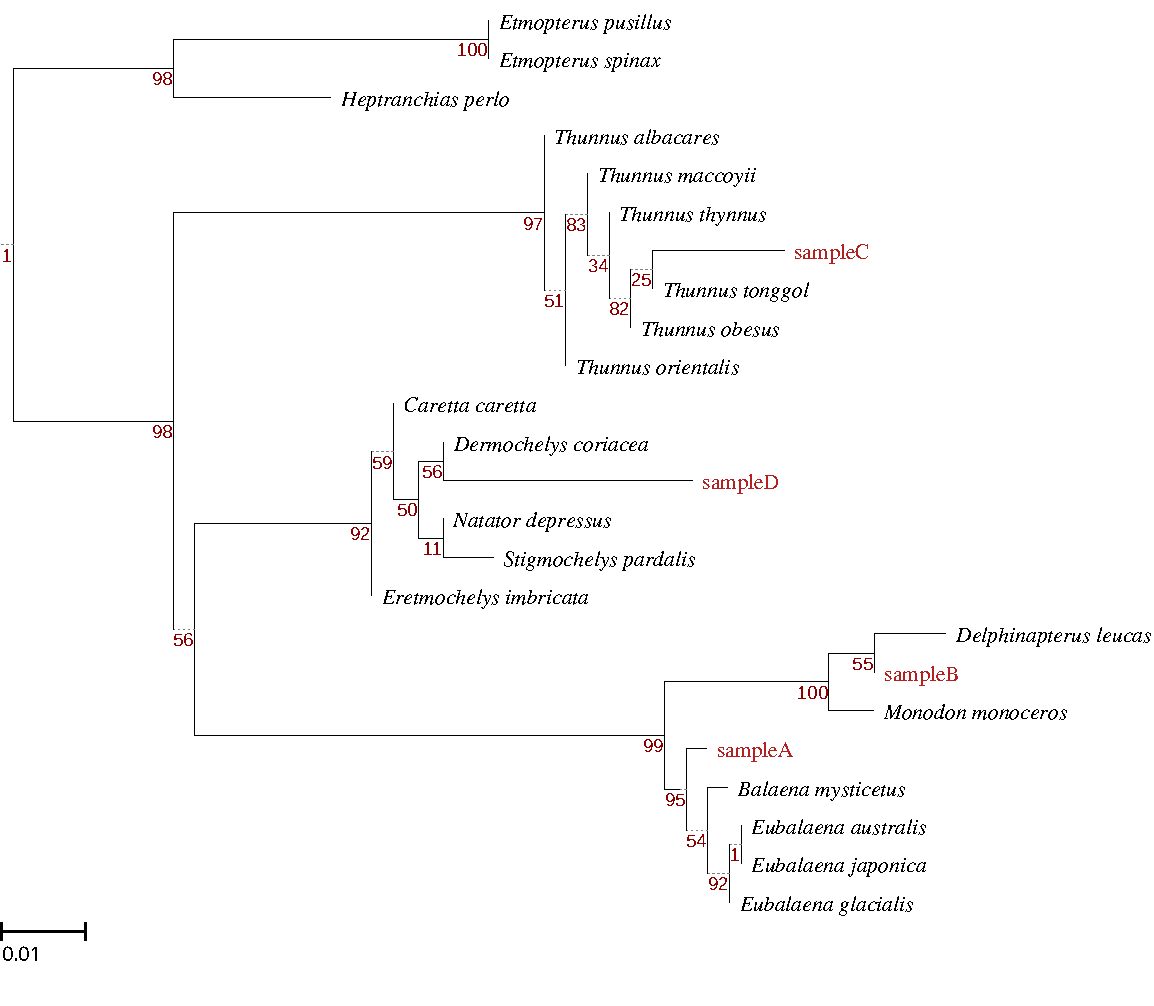
\includegraphics[width=\linewidth, frame]{figures/final_tree.pdf}
	\captionsetup{justification=centering}
	\caption{Phylogenetic tree with placement of unknown meat samples and closest BLAST hits. Scale bar = 0.01 substitutions per site. Bootstrap support shown at nodes.}
	\label{fig:main_tree}
\end{figure}
 
\par Sample A placement was strongly supported within Balaenidae (95\%), but species level resolution was poor. BLAST consistently returned \textit{Eubalaena japonica} as the top hit with a high percentage identity across all parts, suggesting North Pacific right whale as the leading candidate.
\par Sample B placement within Monodontidae was fully supported (100\%), but internal support was weak (55\%). Only \textit{Delphinapterus leucas} and \textit{Monodon monoceros} exist in this family, therefore sample B represents one of these species.
\par Sample C placement was strongly supported within \textit{Thunnus} (97\%), with low-moderate internal node support. BLAST suggested \textit{Thunnus thynnus}, but this is not confirmed by the phylogeny. Sample C may only be assigned to the \textit{Thunnus} genus.
\par Sample D placement within Testudines was strongly supported (92\%), with low support within (11-59\%). Sample D clustered with \textit{Dermochelys coriacea}, consistent with BLAST, suggesting Leatherback sea turtle as the leading candidate.


\section*{Discussion} % 469 WORDS
Order level placement was strongly supported with confident assignment to major vertebrate groups. However, species confidence was low and relied on BLAST compliance with phylogeny for candidate species proposals.
\par The COI fragment for barcoding is $\approx$ 650bp which makes species inference sensitive to sequencing errors, with low quality reads providing limited phylogenetic signal \citep{ahmed2022pragmatic}. FastQC \citep{fastqc} showed low quality calls within all samples, reducing usable bases and likely weakening discriminatory power and reducing bootstrap support. Exploratory alignment (Fig~\ref{fig:needleman}) indicated a potential sequencing misread leading to the apparent frame shift in Fig.~\ref{fig:supermatrix}. Adding one ambiguous base increased sample D/\textit{Dermochelys coriacea} clade support from 56\% to 72\% (Figs.~\ref{fig:supermatrix2}, \ref{fig:tree_pdf2}), illustrating the impact of data quality on phylogenetic confidence. Furthermore, reference sequences from GenBank do not require strict validation and must be interpreted cautiously for species identification \citep{dawnay2007validation, meiklejohn2019assessment}. 
\par Sample A candidate, \textit{Eubalaena japonica}, is listed as `Endangered' \citep{eubalaena}. Presence of this sample raises serious conservation concerns if confirmed, and could reflect trade of a vulnerable whale species. Both sample B candidates are listed under `Least Concern' \citep{monodon, delphinapterus}. Their presence may indicate by-catch from fisheries in or near conservation sites, but without sample origin these implications cannot be assessed fully. \textit{Thunnus} assessments range from `Least Concern' (\textit{Thunnus albacares}) to `Endangered' (\textit{Thunnus maccoyii}) \citep{albacares, maccoyii}. Without species level identification the conservation implications of sample C cannot be assessed. Sample D candidate, \textit{Dermochelys coriacea}, is listed as `Vulnerable' \citep{dermochelys}. This species inhabits protected areas across its range, as such the presence of this sample raises conservation concerns and may reflect illegal trade, depending on the origin of the sample.
\par Overall, COI barcoding here resolved order and family level identity but lacked species level resolution. Longer barcode regions and multiple reads of sample sequences could reduce misreads while increasing resolution among recently diverged species. The use of curated reference databases, such as BOLD, would increase confidence in reference sequences \citep{meiklejohn2019assessment}. These suggestions will allow more confident conservation claims for the meat samples. Nevertheless, the detection of candidate species from undocumented meat illustrates the value of DNA barcoding in the context of the illegal wildlife trade. 


%%%%%%%%%%%%%%%%%%%%%%%%%%%%%%%% check ordering for years and surnames etc.
\bibliography{references}
%%%%%%%%%%%%%%%%%%%%%%%%%%%%%%%%


\section*{Supplementary Data}
Supplementary data and scripts are found in the following GitHub repository: \url{https://github.com/archiebenn/BIOLM0051_analysis.git}

\newpage
\section*{Appendix: Exploratory Figures}
\vspace{2em}
%%%%%%%%%%%%%%%
% Bash block
%%%%%%%%%%%%%%%
\begin{figure}[H]
\centering	
\begin{minted}[fontsize=\small, frame=single, framesep=1.5mm, bgcolor=gray!1]{text}
Dermochelys_c    441 CACCTAGCTGGTGTTTCATCAATTTTAGGAGCTATTAACTTCATTACTAC    490
                     |||||||||||||||||||||||||||||||||||| |||||||||||||
sampleD_part1    451 CACCTAGCTGGTGTTTCATCAATTTTAGGAGCTATT-ACTTCATTACTAC    499
\end{minted} 
\raisebox{2em}{\hspace{6.55cm}$\big\uparrow$}
\vspace{-2em}
\captionsetup{justification=centering}
\caption{MAFFT \cite{mafft} Needleman-Wunsch alignment. Gap indicates a possible misread during sequencing.}
\label{fig:needleman}
\end{figure}
\vspace{5em}

\begin{figure}[H]
	\centering
	\begin{texshade}{figures/sampleD_supermatrix.afa}
		\hideseq{1,3,6,7,8,9,10,11,12,15,16,17,18,19,20,21,22,23}
		\conservedresidues{Black}{Yellow}{upper}{filled}
		\allmatchresidues{Black}{SeaGreen}{upper}{filled}
		\threshold[85]{50}
		\setends{1}{145..179}
		\feature{top}{1}{0..171}{--,}{Part 1}
		\feature{top}{1}{172..184}{,--}{Part 2}
		\feature{bottom}{1}{159..171}{brace}{Altered protein sequence follows conserved region closely}
		\hideconsensus
		\showlegend
	\end{texshade}
	\captionsetup{justification=centering}
	\caption{Alignment after inserting one ambiguous base (N) in \texttt{sampleD\_part1}}
	\label{fig:supermatrix2}
\end{figure}

\begin{figure}[H]
	\centering
	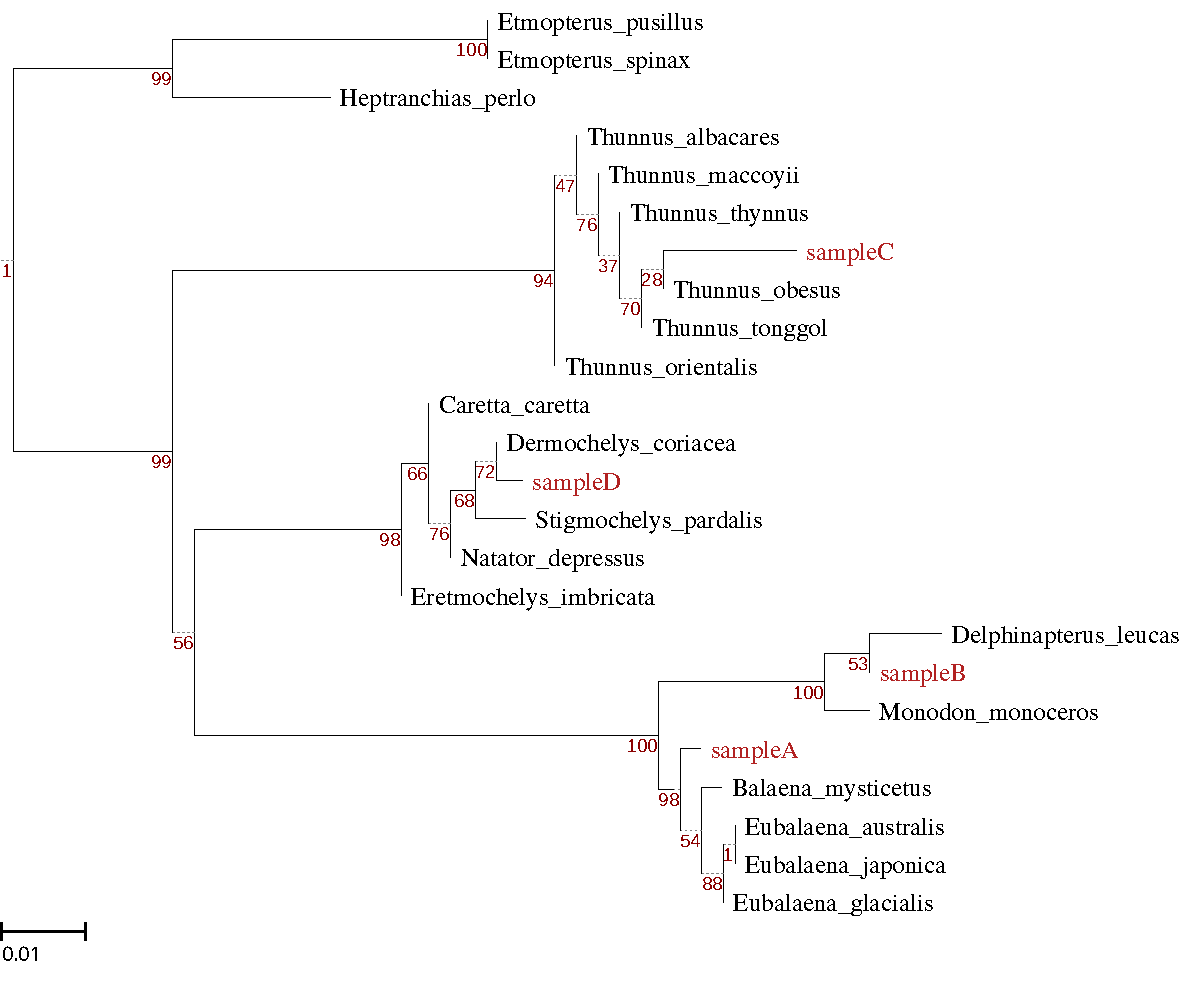
\includegraphics[width=\linewidth, frame]{figures/final_tree_D_branch.pdf}
	\captionsetup{justification=centering}
	\caption{Phylogenetic tree resulting from altered alignment (Fig. \ref{fig:supermatrix2}).}
	\label{fig:tree_pdf2}
\end{figure}



\end{document}